\documentclass{article}
\usepackage{tikz}
\setlength{\parindent}{1cm}
\usepackage[margin=1.25in]{geometry}
\usepackage{amsmath, amssymb}
\usepackage{graphicx}

\begin{document}
	
	\tableofcontents
	\section{Previous lunar missions}
	\section{Going to the moon now}
	\subsection{The direct way}
	
	
	\begin{center}
		{\Huge Big Centered Text}
	\end{center}
	
	Here is a paragraph. Notice that the paragraph was indented even though I didn't tell
	\LaTeX{} to indent. This is because indentation is automatic.
	
	Notice that there is a black line of text between this paragraph and the previous one. 
	Without that blank line, \LaTeX{} will not start a new paragraph.
	
	\noindent To skip the indentation for a single paragraph, you can use  the \verb|\noindent|
	command. If you wanted to skip indentations for the entire document, you can set the 
	indentation size to zero.
	
	\setlength{\parindent}{15pt}
	
	The standard indentation is 15pt. Notice that this is smaller than the 1cm indentation
	that was created in the preamble. The default size is usually fine and there's usually
	no reason to change it.
	
	\begin{align}
		f(x) & = a_2 x^2 + a_1 x + a_0 \\
		& = x^2 + 4x - 5
	\end{align}
	
	\begin{align}
		f(x) & = a_2 x^2 + a_1 x + a_0 \nonumber \\
		     & = x^2 + 4x - 5
	\end{align}

	\begin{align*}
		2x + 1 & = 9 	& 	3y - 2 & = -5 	& -5z + 8 & = 3 \\
		2x & = 8 	&     3y & = -3 	&     -5z & = -5 \\ 
		x & = 4		& 	y & = -1	& 	z & = -1
	\end{align*}

	Notice that by substitution we get the equation $f(x) = x^2 + 4x - 5$. This is the
	quadratic function in the variable $x$, and we can identify the vertex by completing 
	the square...
	
	\begin{align*}
		\sum_{n=1}^\infty \frac{1}{n^2} = \frac{\pi^2}{6}	
	\end{align*}

	\begin{align}
		\left(	\sum_{n=0}^N	\left(  \frac{1}{a+b}	\right)^2	\right)^2
	\end{align}

	\begin{align*}
		n = ab \text{ where } a \text{ and } b \text{ are natural numbers}
	\end{align*}

\begin{align*}
	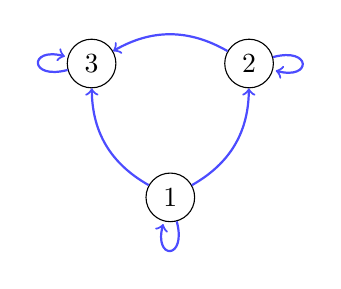
\begin{tikzpicture}
		%%%% Add nodes for each number
		\node[shape=circle,draw] (1) at (0,0) {1};
		\node[shape=circle,draw] (2) at (1,1.7) {2};
		\node[shape=circle,draw] (3) at (-1,1.7) {3};
		%%%% Add edges between nodes
		\draw[->,color=blue!70,thick] (1) to[bend right] (2);
		\draw[->,color=blue!70,thick] (1) to[bend left] (3);
		\draw[->,color=blue!70,thick] (2) to[bend right] (3);
		%%%% Add self referential edges
		\draw[->,color=blue!70,thick] (1) edge[loop below] (1);
		\draw[->,color=blue!70,thick] (2) edge[loop right] (2);
		\draw[->,color=blue!70,thick] (3) edge[loop left] (3);
	\end{tikzpicture}	
\end{align*}	

\begin	

		
\end{document}